\section{Sistemi Elementari}

I sistemi elementari sono una rappresentazione astratta per modellare sistemi dinamici utilizzando le reti di Pedri. Formalmente, un sistema elementare $\Sigma = (B, E, F, c_{in})$ è definito da una rete elementare $N = (B, E, F)$ e da un caso iniziale $c_{in} \subseteq B$.

\subsection{Reti Elementari}
$N = (B, E, F)$ è una \textbf{rete} se e solo se:
\begin{itemize}
	\item $B$ è un insieme finito di condizioni (vere o false).

	\item $E$ è un insieme finito di eventi (transizioni locali).
	\item $F \subseteq B (B \times E) \cup (E \times B)$ tale che $dom(F) \cup ran(F) = B \cup E$, ovvero non ci sono elementi isolati.
\end{itemize}
con $B \cap E = \emptyset$, e $B \cup E \neq \emptyset$
\\
\\
Sia $x \in B \cup E = X$, denotiamo con
\begin{itemize}
	\renewcommand\labelitemi{} % Remove bullet for the first level
	\item $\bullet x = \{ y \in X | (y, x) \in F \}$ pre-elementi di $x$
	\item $x \bullet = \{ y \in X | (x, y) \in F \}$ post-elementi di $x$
	\item Sia $A \subseteq B \cup E$, allora $\bullet A = \bigcup_{x \in A}{\bullet x}$, $A \bullet = \bigcup_{x \in A}{x \bullet}$
\end{itemize}
\vspace{1em}
\noindent
La rete $N = (B, E, F)$ descrive la \textbf{struttura statica} del sistema. Il comportamento è definito attraverso le nozioni di \textbf{caso} e \textbf{regola di scatto}.
\\
\\
Un \textbf{caso} è un insieme di condizioni \(C \subseteq B\) che descrive lo stato corrente di un sistema. Le condizioni in \(C\) rappresentano gli \textbf{stati locali} attualmente veri, che insieme determinano lo \textbf{stato globale} del sistema.

\begin{center}
	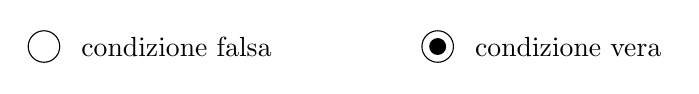
\begin{tikzpicture}
		\draw (0,0) circle (0.2cm) node[right=1em] {condizione falsa};
		\draw[fill=black] (5,0) circle (0.1cm) node[right=1em] {condizione vera};
		\draw (5,0) circle (0.2cm);
	\end{tikzpicture}
\end{center}

\noindent
Una \textbf{regola di scatto} descrive come un evento modifica lo stato del sistema.\\
Sia $N = (B, E, F)$ una rete elementare, e $c \subseteq B$. L'evento $e \in E$ è \textbf{abilitato} (può occorrere) in  $c$, denotato con $c[e$, se e solo se:
\[
	\bullet e \subseteq c \ \wedge \ e \bullet \cap c = \emptyset
\]

\noindent
Abbiamo che un evento è completamente caratterizzato dai cambiamenti che produce negli \textbf{stati locali}. Tali cambiamenti sono \textbf{indipendenti} dalla particolare configurazione in cui l'evento occorre. In pratica, l'evento "guarda" solo le sue pre e post condizioni.

\subsection{Reti Semplici e Reti Pure}
Sia $N = (B, E, F)$ una rete elementare, allora:
\begin{itemize}
	\item N è \textbf{semplice} se e solo se
	      \[
		      \forall x, y \in B \cup E,
		      \quad (\bullet x = \bullet y \ \wedge \ x \bullet = y \bullet) \implies x = y
	      \]
	      \textit{Esempio di rete non-semplice}:
	      \begin{center}
		      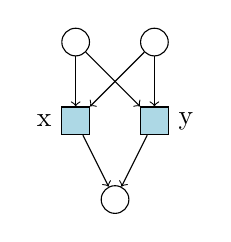
\begin{tikzpicture}
			      \node[shape = circle, draw,minimum size=1em] (B) at (1, -1){};
			      \node[shape = circle, draw,minimum size=1em] (C) at (2, -1){};

			      \node[shape=rectangle, draw, fill=LightBlue, minimum size=1em, label=left:x] (x) at (1, -2){};
			      \node[shape=rectangle, draw, fill=LightBlue, minimum size=1em, label=right:y] (y) at (2, -2){};

			      \node[shape = circle, draw, minimum size=1em] (D) at (1.5, -3){};

			      \draw[->] (B) to (x);
			      \draw[->] (B) to (y);
			      \draw[->] (x) to (D);
			      \draw[->] (y) to (D);
			      \draw[->] (C) to (x);
			      \draw[->] (C) to (y);
		      \end{tikzpicture}
	      \end{center}
	\item $N$ è \textbf{pura} se e solo se
	      \[
		      \forall e \in E, \quad \bullet e \cap e \bullet = \emptyset
	      \]
	      \textit{Esempio di rete non-pura}:
	      \begin{center}
		      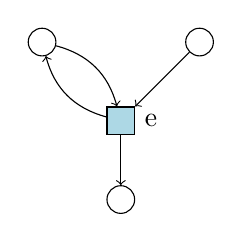
\begin{tikzpicture}
			      \node[shape=rectangle, draw, minimum size=1em, fill=LightBlue, label=right:e] (e) at (1, -1){};
			      \node[shape = circle, draw,minimum size=1em] (A) at (0, 0){};
			      \node[shape = circle, draw,minimum size=1em] (B) at (2, 0){};
			      \node[shape = circle, draw, minimum size=1em] (C) at (1, -2){};

			      \draw[->] (A) to[bend left] (e);
			      \draw[->] (e) to[bend left] (A);
			      \draw[->] (B) to (e);
			      \draw[->] (e) to (C);
		      \end{tikzpicture}
	      \end{center}
\end{itemize}

\subsection{Eventi Indipendenti ed Eventi Concorrenti}
Sia $N = (B, E, F)$ una rete elementare, $U \subseteq E$, e $c, c_1, c_2 \subseteq B$, allora:
\begin{itemize}
	\item $U$ è un insieme di \textbf{eventi indipendenti} se e solo se
	      \[
		      \forall e_1, e_2 \in U, \quad e_1 \neq e_2
		      \implies
		      (\bullet e_1 \cup e_1 \bullet) \cap (\bullet e_2 \cup e_2 \bullet)
		      =
		      \emptyset
	      \]
	      ovvero non hanno \textbf{nessuna} pre o post condizione in comune
	\item $U$ è un \textbf{passo abilitato} se e solo se
	      \[
		      U \text{ insieme di eventi indipendenti} \quad \wedge \quad \forall e \in U, \ c[e >
	      \]
	      ovvero è un insieme di eventi concorrenti
	\item $U$ è un \textbf{passo da $c_1$ a $c_2$}, scritto $c_1[U > c_2$ se e solo se
	      \[
		      c_1[U >
		      \quad \wedge \quad
		      c_2 = (c_1 \setminus \prescript{\bullet}{}{U}) \cup U^\bullet
	      \]
\end{itemize}

\subsection{Grafo dei casi raggiungibili}

L'insieme dei \textbf{casi raggiungibili} $C_\Sigma$ del sistema elementare $\Sigma = (B, E, F, c_{in})$ è il più piccolo sottoinsieme di $2^B$ tale che
\begin{itemize}
	\renewcommand\labelitemi{} % Remove bullet for the first level
	\item $c_{in}  \in C_\Sigma$
	\item se $c \in C_\Sigma, U \subseteq E, c' \subseteq B$ sono tali che $c[U > c'$, allora $c' \in C_\Sigma$
\end{itemize}
\vspace{1em}
$U_\Sigma$ è l'\textbf{insieme dei passi} di $\Sigma$ tale che
\[
	U_\Sigma = \{ U \subseteq E | \exists c, c' \in C_\Sigma : c[U | c' \}
\]

\noindent
Il comportamento di un sistema elementare $\Sigma = (B, E, F, c_{in})$ può essere rappresentato dal suo \textbf{grafo dei casi}. Il grafo dei casi di $\Sigma$ è il \textbf{sistema di transizioni etichettato} $CG_\Sigma = (C_\Sigma, U_\Sigma, A, c_{in})$ dove:
\begin{itemize}
	\item $C_\Sigma$ è l'insieme dei nodi del grafo (gli stati globali)
	\item $U_\Sigma$ è l'alfabeto
	\item $A$ è l'insieme di archi etichettati\\
	      $A = \{ (c, U, c') | c, c' \in C_\Sigma, U \in U_\Sigma, c[U > c' \}$
\end{itemize}

\noindent
Esempio di sistema $\Sigma$ e il suo grafo dei casi $CG_\Sigma$:

\begin{center}
	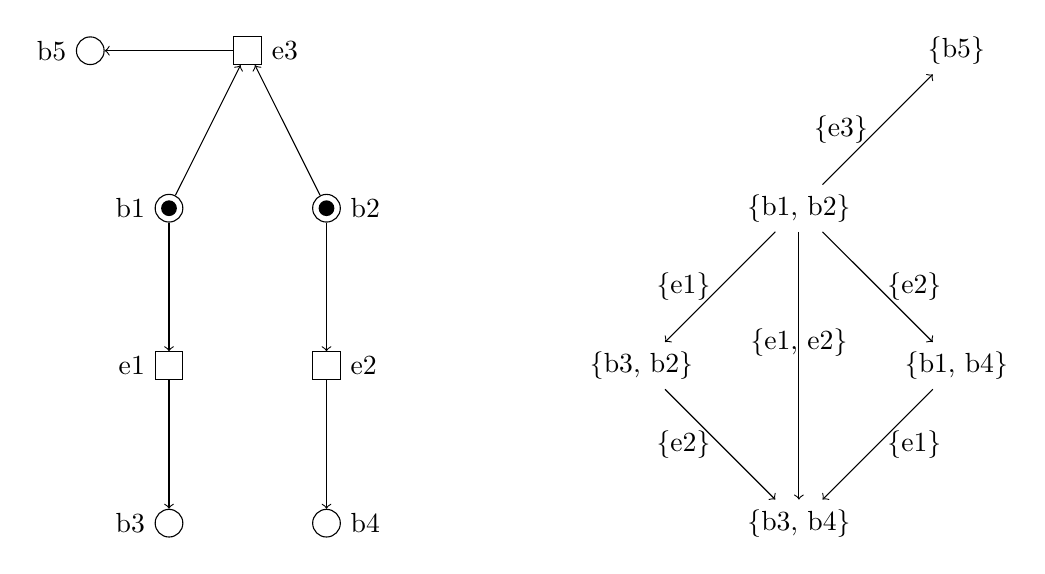
\begin{tikzpicture}
		% Sistema
		\node[shape=rectangle, draw, minimum size=1em, label=right:e3] (e3) at (-7, 2){};
		\node[shape = circle, draw, minimum size=1em, label=left:b5] (b5) at (-9, 2){};

		\node[shape = circle, draw, minimum size=1em, label=left:b1] (b1) at (-8, 0){};
		\fill (-8,0) circle (1mm);
		\node[shape = circle, draw, minimum size=1em, label=right:b2] (b2) at (-6, 0){};
		\fill (-6,0) circle (1mm);

		\node[shape=rectangle, draw, minimum size=1em, label=left:e1] (e1) at (-8, -2){};
		\node[shape=rectangle, draw, minimum size=1em, label=right:e2] (e2) at (-6, -2){};

		\node[shape = circle, draw, minimum size=1em, label=left:b3] (b3) at (-8, -4){};
		\node[shape = circle, draw, minimum size=1em, label=right:b4] (b4) at (-6, -4){};

		\draw[->] (e3) to (b5);
		\draw[->] (b1) to (e3);
		\draw[->] (b2) to (e3);
		\draw[->] (b1) to (e1);
		\draw[->] (b2) to (e2);
		\draw[->] (e1) to (b3);
		\draw[->] (e2) to (b4);


		% Grafo dei casi
		\node (b1b2) at (0, 0){\{b1, b2\}};
		\node (b3b2) at (-2, -2){\{b3, b2\}};
		\node (b1b4) at (2, -2){\{b1, b4\}};
		\node (b3b4) at (0, -4){\{b3, b4\}};
		\node (b5) at (2, 2){\{b5\}};

		\draw[->] (b1b2) edge node[left] {\{e1\}} (b3b2);
		\draw[->] (b1b2) edge node[right] {\{e2\}} (b1b4);
		\draw[->] (b3b2) edge node[left] {\{e2\}} (b3b4);
		\draw[->] (b1b4) edge node[right] {\{e1\}} (b3b4);
		\draw[->] (b1b2) edge node[above] {\{e1, e2\}} (b3b4);
		\draw[->] (b1b2) edge node[left] {\{e3\}} (b5);
	\end{tikzpicture}
\end{center}

\subsection{Diamond Property}
Sia $\Sigma = (B, E, F, c_{in})$ un sistema elementare, $CG_\Sigma = (C_\Sigma, U_\Sigma, A, c_{in})$ il suo grafo dei casi, $U_1, U_2 \in U_\Sigma : U_1 \cap U_2 = \emptyset$, $U_1 \neq \emptyset$, $U_2 \neq \emptyset$, e $c_1, c_2, c_3, c_4 \in C_\Sigma$, allora vale:
\begin{center}
	\begin{tikzpicture}
		% Not diamond
		\node (c1) at (-7, 0){c1};
		\node (c2) at (-9, -2){c2};
		\node (c4) at (-5, -2){c4};
		\node (c3) at (-7, -4){c3};

		\draw[->] (c1) edge node[left] {U1} (c2);
		\draw[->] (c1) edge node[right] {U2} (c4);
		\draw[->] (c2) edge node[left] {U2} (c3);

		% Middle arrow

		\draw[<->, ultra thick] (-4, -2) to (-3, -2);

		% Diamond
		\node (c1) at (0, 0){c1};
		\node (c2) at (-2, -2){c2};
		\node (c4) at (2, -2){c4};
		\node (c3) at (0, -4){c3};

		\draw[->] (c1) edge node[left] {U1} (c2);
		\draw[->] (c1) edge node[right] {U2} (c4);
		\draw[->] (c2) edge node[left] {U2} (c3);
		\draw[->] (c4) edge node[right] {U1} (c3);
		\draw[->] (c1) edge node[above] {U1 $\cup$ U2} (c3);
	\end{tikzpicture}
\end{center}

\textbf{Dimostrazione slide lez2 p23}

\subsection{Grafo dei casi sequienziale}
Il grafo dei casi sequenziali di $\Sigma = (B, E, F, c_{in})$ è $SCG_\Sigma = (C_\Sigma, E, A, c_{in})$ dove:
\[
	A = \{ (c, e, c') | c, c' \in C_\Sigma, e \in E : c[e > c' \}
\]
\noindent
Per la diamond property, nei sistemi elementari il grafo dei casi e il grafo dei casi sequenziali sono \textbf{sintatticamente equivalenti} (ovvero possono essere ricavati l'uno dall'altro).
Questo implica che due sistemi elementari hanno grafi dei casi isomorfi se e solo se hanno grafi dei casi sequenziale isomorfi.

\subsection{Isomorfismo tra Sistemi di Transizioni Etichettati}
Siano $A_1 = (S_1, E_1, T_1, s_{01})$ e $A_2 = (S_2, E_2, T_2, s_{02})$ sistemi di transizioni etichettati,
$\alpha : S_1 \to S_2$ e $\beta : E_1 \to E_2$ \textbf{mappe biunivoche}, allora:
\[
	\langle \alpha, \beta \rangle : A_1 = (S_1, E_1, T_1, s_{01}) \to A_2 = (S_2, E_2, T_2, s_{02})
\]
\noindent
è un \textbf{isomorfismo} se e solo:
\begin{itemize}
	\item $\alpha (s_{01}) = s_{02}$
	\item $\forall s, s' \in S_1, \forall e \in E_1, \quad (s, e, s') \in T_1 \iff (\alpha(s), \beta(e), \alpha(s')) \in T_2$
\end{itemize}

\noindent
A questo punto possiamo definire l'equivalenza tra sistemi. Due sistemi $\Sigma_1$ e $\Sigma_2$ sono \textbf{equivalenti} se e solo se hanno grafi dei casi sequenziali (e quindi anche grafi dei casi) \textbf{isomorfi}.

\subsection{Contatti}

Sia $\Sigma = (B, E, F, c_{in})$ un sistema elementare, $e \in E$, $c \in C_\Sigma$. Abbiamo che la coppia $(e, c)$ è un \textbf{contatto} se e solo se:
\[
	\prescript{\bullet}{}{e} \subseteq c \ \wedge \ e^\bullet \cap c \neq \emptyset
\]
\noindent
Ovvero tutte le pre-condizioni di $e$ sono vere, ma non tutte le sue post-condizioni sono false.
\\
\\
Un sistema elementare $\Sigma = (B, E, F, c_{in})$ è \textbf{senza contatti} se e solo se
\[
	\forall e \in E, \forall c \in C_\Sigma,
	\quad
	\prescript{\bullet}{}{e} \subseteq c \implies e^\bullet \cap c = \emptyset
\]

\noindent
È possibile trasformare un sistema elementare $\Sigma$ con contatti in un sistema elementare $\Sigma'$ che sia senza contatti, senza modificarne il comportamento. Aggiungendo a $\Sigma$ il \textbf{complemento} di ogni condizione si ottiene un sistema $\Sigma'$ con grafo dei casi isomorfo a quello di $\Sigma$. Il complemento di una condizione si ottiene negando la condizione stessa e invertendo il senso delle frecce che la collegano.
\\
\\
Se abbiamo un sistema senza contatti, per verificare che un evento $e$ sia abilitato in un caso raggiungibile $c$, è sufficiente verificare che le precondizioni di $e$ siano vere:
\[
	c[e> \quad \iff \quad \prescript{\bullet}{}{e} \subseteq c
\]

\subsection{Situazioni fondamentali}
Sia $\Sigma = (B, E, F, c_{in})$ un sistema elementare, $c \in C_\Sigma$, $e_1, e_2 \in E$, abbiamo che:

\begin{itemize}
	\item $e_1$ e $e_2$ sono in \textbf{sequenza} in $c$ se e solo se
	      \[
		      c[e_1 >
		      \quad \wedge \quad
		      \neg c[e_1
		      \quad \wedge \quad
		      c[e_1 e_2 > (c[e_1 > c'[e_2)
	      \]
	      \begin{center}
		      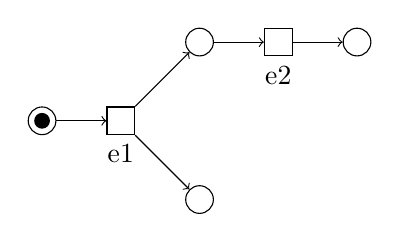
\begin{tikzpicture}
			      \node[shape=circle, draw, minimum size=1em] (b1) at (0, 0){};
			      \node[shape=circle, draw, minimum size=1em] (b2) at (2, 1){};
			      \node[shape=circle, draw, minimum size=1em] (b3) at (2, -1){};
			      \node[shape=circle, draw, minimum size=1em] (b4) at (4, 1){};
			      \node[shape=rectangle, draw, minimum size=1em, label=below:e1] (e1) at (1, 0){};
			      \node[shape=rectangle, draw, minimum size=1em, label=below:e2] (e2) at (3, 1){};


			      \fill (b1) circle (1mm);

			      \draw[->] (b1) to (e1);
			      \draw[->] (e1) to (b2);
			      \draw[->] (e1) to (b3);
			      \draw[->] (b2) to (e2);
			      \draw[->] (e2) to (b4);
		      \end{tikzpicture}
	      \end{center}

	\item $e_1$ e $e_2$ sono \textbf{concorrenti} in $c$ se e solo se
	      \[
		      c[\{ e_1, e_2 \}
	      \]
	      \begin{center}
		      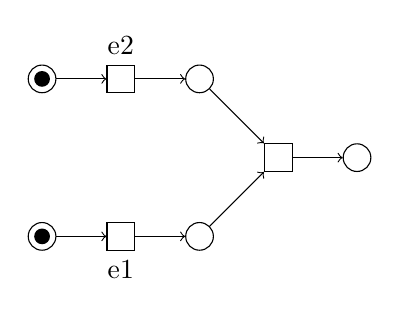
\begin{tikzpicture}
			      \node[shape=circle, draw, minimum size=1em] (b1) at (0, 0){};
			      \node[shape=circle, draw, minimum size=1em] (b2) at (0, -2){};
			      \node[shape=rectangle, draw, minimum size=1em, label=above:e2] (e2) at (1, 0){};
			      \node[shape=rectangle, draw, minimum size=1em, label=below:e1] (e1) at (1, -2){};
			      \node[shape=circle, draw, minimum size=1em] (b3) at (2, 0){};
			      \node[shape=circle, draw, minimum size=1em] (b4) at (2, -2){};
			      \node[shape=rectangle, draw, minimum size=1em] (e3) at (3, -1){};
			      \node[shape=circle, draw, minimum size=1em] (b5) at (4, -1){};


			      \fill (b1) circle (1mm);
			      \fill (b2) circle (1mm);

			      \draw[->] (b1) to (e2);
			      \draw[->] (b2) to (e1);
			      \draw[->] (e1) to (b4);
			      \draw[->] (e2) to (b3);
			      \draw[->] (b3) to (e3);
			      \draw[->] (b4) to (e3);
			      \draw[->] (e3) to (b5);
		      \end{tikzpicture}
	      \end{center}

	\item $e_1$ e $e_2$ sono in \textbf{conflitto} in $c$ se e solo se
	      \[
		      c[e_1>
		      \quad \wedge \quad
		      c[e_2>
		      \quad \wedge \quad
		      \neg c [ \{ e_1, e_2 \} >
	      \]
	      ovvero sono entrambi abilitati, ma l'occorrenza di uno disabilita l'altro:
	      \begin{center}
		      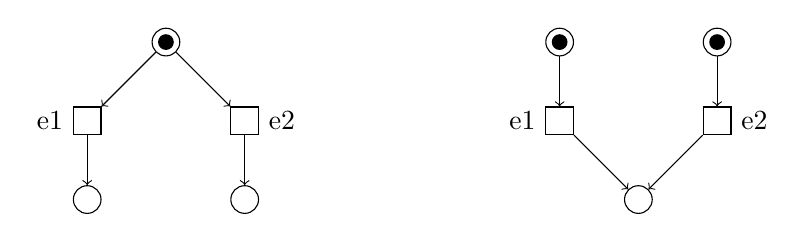
\begin{tikzpicture}
			      % forward
			      \node[shape=circle, draw, minimum size=1em] (b1) at (0, 0){};
			      \node[shape=rectangle, draw, minimum size=1em, label=left:e1] (e1) at (-1, -1){};
			      \node[shape=rectangle, draw, minimum size=1em, label=right:e2] (e2) at (1, -1){};
			      \node[shape=circle, draw, minimum size=1em] (b2) at (-1, -2){};
			      \node[shape=circle, draw, minimum size=1em] (b3) at (1, -2){};
			      \fill (b1) circle (1mm);

			      \draw[->] (b1) to (e1);
			      \draw[->] (b1) to (e2);
			      \draw[->] (e1) to (b2);
			      \draw[->] (e2) to (b3);


			      % backward 
			      \node[shape=circle, draw, minimum size=1em] (b10) at (5, 0){};
			      \node[shape=circle, draw, minimum size=1em] (b11) at (7, 0){};
			      \node[shape=rectangle, draw, minimum size=1em, label=left:e1] (e10) at (5, -1){};
			      \node[shape=rectangle, draw, minimum size=1em, label=right:e2] (e11) at (7, -1){};
			      \node[shape=circle, draw, minimum size=1em] (b12) at (6, -2){};
			      \fill (b10) circle (1mm);
			      \fill (b11) circle (1mm);

			      \draw[->] (b10) to (e10);
			      \draw[->] (b11) to (e11);
			      \draw[->] (e10) to (b12);
			      \draw[->] (e11) to (b12);
		      \end{tikzpicture}
	      \end{center}
	      Inoltre, $e_1$ e $e_2$ sono in \textbf{conflitto strutturale} quando
	      \[
		      \prescript{\bullet}{}{e_1} \cap \prescript{\bullet}{}{e_2} \neq \emptyset
		      \quad \vee \quad
		      e_1^\bullet \cap e_2^\bullet \neq \emptyset
	      \]

	\item Quando c'è un "misto" di concorrenza e conflitto si verifica una \textbf{confusione}, ovvero non è possibile stabilire oggettivamente se si è risolta una confusione.
\end{itemize}

\subsection{Sottorete}
Siano $N = (B, E, F)$ e $N_1 = (B_1, E_1, F_1)$ due reti elementari, allora
\\
\\
$N_1 = (B_1, E_1, F_1)$ è \textbf{sottorete} di $N = B, E, F)$ se e solo se
\begin{itemize}
	\item $B_1 \subseteq B$
	\item $E_1 \subseteq E$
	\item $F_1 = F \cap [(B_1 \times E_1) \cup (E_1 \times B_1) ]$
\end{itemize}

\noindent
$N_1 = (B_1, E_1, F_1)$ è la \textbf{sottorete generata} da $B_1$ se e solo se
\begin{itemize}
	\item $B_1 \subseteq B$
	\item $E_1 = \prescript{\bullet}{}{B_1} \cup B_1^\bullet$
    \item $F_1 = F \cap [(B_1 \times E_1)\cup(E_1 \times B_1)]$
\end{itemize}

\noindent
$N_1 = (B_1, E_1, F_1)$ è la \textbf{sottorete generata} da $E_1$ se e solo se
\begin{itemize}
    \item $B_1 = \prescript{\bullet}{}{E_1} \cup E_1^\bullet$
	\item $E_1 \subseteq E$
    \item $F_1 = F \cap [(B_1 \times E_1)\cup(E_1 \times B_1)]$
\end{itemize}

\subsection{Composizione per Reti di Petri}
Per comporre due reti in modo tale che queste interagiscano abbiamo due modi principali: composizione \textbf{sincrona} e \textbf{asincrona}. Nella composizione sincrona, le due reti hanno un evento in comune. Nella composizione asincrona invece, le due reti hanno una condizione in comune.
\textbf{esercizi slide 3b}
